\documentclass{beamer}
\usepackage[utf8]{inputenc}
\usepackage{caption}
\usepackage{hyperref}
\usepackage{graphicx}
\usepackage{amsmath, amssymb, amsthm}
\usetheme{Warsaw}
\newcommand*{\mdot}{\ensuremath{\ . \ }}


\hypersetup{colorlinks = true}

\title{Isabelle/HOL}
\subtitle{CAS 701 Project Presentation}
\author{Brooks MacLachlan and Nhan Thai}
\date{\today}

\begin{document}

  \frame{\titlepage}

  \begin{frame}
    \frametitle{Proof Assistant}
    \centering
    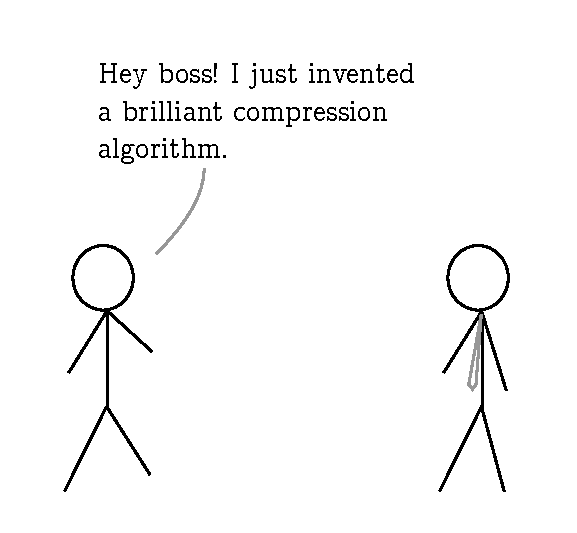
\includegraphics[scale=0.8]{images/1.pdf}
  \end{frame}
  \begin{frame}
    \frametitle{Proof Assistant}
    \centering
    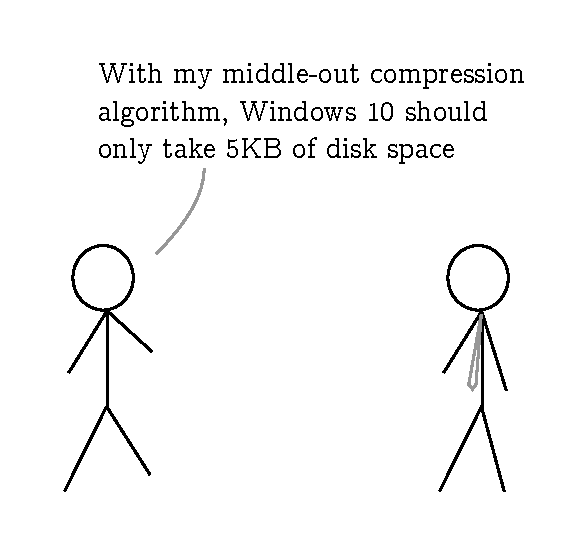
\includegraphics[scale=0.8]{images/2.pdf}
  \end{frame}
  \begin{frame}
    \frametitle{Proof Assistant}
    \centering
    
\includegraphics[scale=0.8]{images/3.pdf}
  \end{frame}
  \begin{frame}
    \frametitle{Proof Assistant}
    \centering
    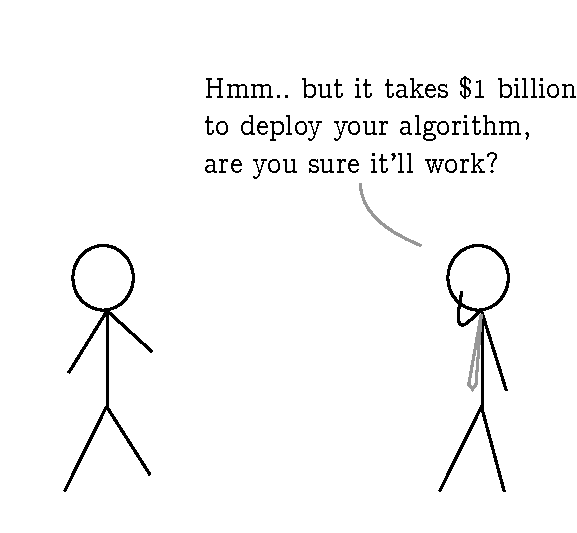
\includegraphics[scale=0.8]{images/4.pdf}
  \end{frame}
  \begin{frame}
    \frametitle{Proof Assistant}
    \centering
    
\includegraphics[scale=0.8]{images/5.pdf}
  \end{frame}
  \begin{frame}
    \frametitle{Proof Assistant}
    \centering
    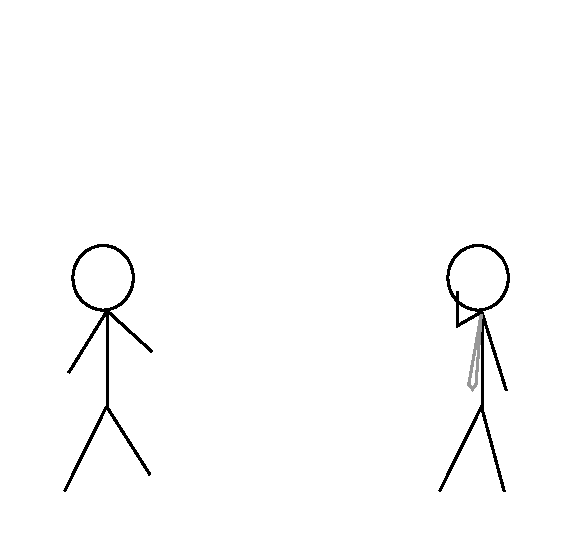
\includegraphics[scale=0.8]{images/6.pdf}
  \end{frame}
  \begin{frame}
    \frametitle{Proof Assistant}
    \centering
    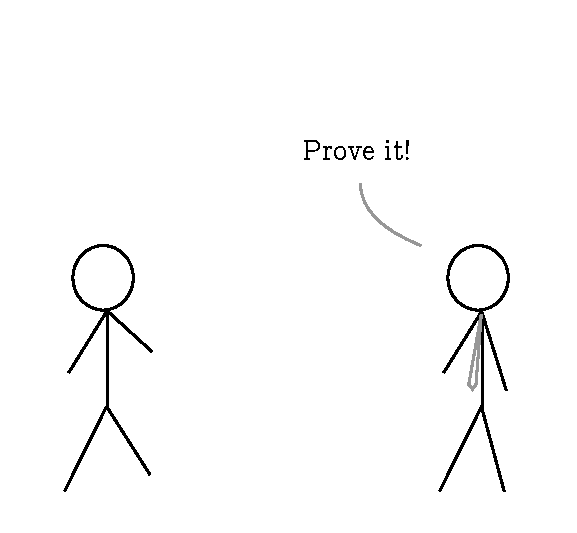
\includegraphics[scale=0.8]{images/7.pdf}
  \end{frame}
  \begin{frame}
    \frametitle{Proof Assistant}
    \centering
    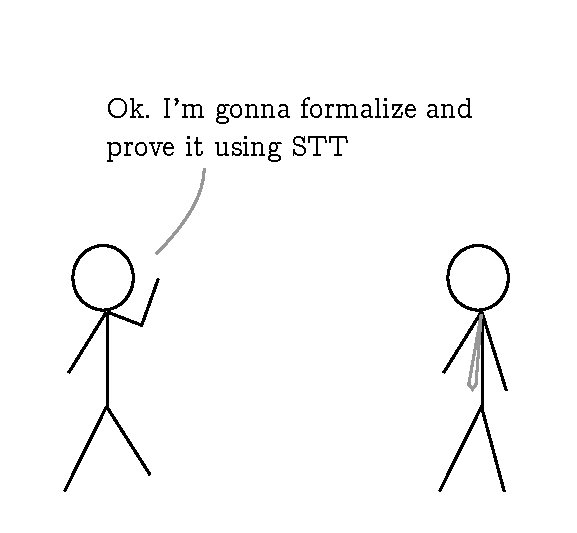
\includegraphics[scale=0.8]{images/8.pdf}
  \end{frame}
  \begin{frame}
    \frametitle{Proof Assistant}
    \textbf{Formalize and proof}: \\
    Natural number:
    \begin{itemize}
      \item $\tau(0) = \iota, \tau(S) = \iota \rightarrow \iota, \tau(nat) = \iota \rightarrow *$
      \item $\forall x : \iota \mdot nat(x) \Rightarrow nat(S(x))$
      \item $\forall x : \iota \mdot nat(x) \Rightarrow  0 \neq S(x)$
      \item $\forall x, y : \iota \mdot nat(x) \land nat(y) \Rightarrow S(x) = S(y) \equiv x = y$
      \item $\forall P : \iota \rightarrow * \mdot P(0)
      \land (\forall x : \iota \mdot nat(x) \Rightarrow P(x) \Rightarrow P(S(x)))
      \Rightarrow \forall x : \iota \mdot nat(x) \Rightarrow P(x)$
      \item \ldots
    \end{itemize}
    Binary tree:
    \begin{itemize}
      \item $\tau(Leaf) = \iota \rightarrow \iota,
      \tau(Branch) = \iota \rightarrow \iota \rightarrow \iota \rightarrow \iota,
      \tau(bin) = \iota \rightarrow *$
      \item $\forall x, y, a, b : \iota \mdot bin(x) \land bin(y) \Rightarrow Leaf(a) \neq Branch(b, x, y)$
      \item \ldots
    \end{itemize}
  \end{frame}
  \begin{frame}
    \frametitle{Proof Assistant}
    Order:
    \begin{itemize}
      \item \ldots
    \end{itemize}
    Compressing algorithm:
    \begin{itemize}
      \item \ldots
    \end{itemize}
  \end{frame}
  \begin{frame}
    \frametitle{Proof Assistant}
    \begin{itemize}
      \item 100 pages later \ldots
      \item $size(compress(windows10)) \leq 5$ (Q.E.D)
    \end{itemize}
    \textbf{End} \\
  \end{frame}
  \begin{frame}
    \frametitle{Proof Assistant}
    \begin{itemize}
      \item<1-> Hand-written proof
      \begin{itemize}
        \item Long and tedious
        \item Repetitive concepts
        \item Error-prone
      \end{itemize}
      \item<2-> $\Rightarrow$ Let the computer do what can be automated
    \end{itemize}

  \end{frame}

  \begin{frame}
    \frametitle{Isabelle/HOL}
    \begin{itemize}
      \item<1-> Simple Type Theory
      \item<2-> Extensible types of individuals
      \begin{itemize}
        \item No need for a predicate ($\iota \rightarrow *$) for each kind of individual
        \item Built-in: \textit{int}, \textit{real}, \textit{nat}, \ldots
        \item User-defined inductive types
        \item Type polymorphism: \textit{int list}, \textit{'a tree}, \textit{'a list}, \ldots
      \end{itemize}
    \end{itemize}
  \end{frame}

  \begin{frame}
    \frametitle{User-defined type}
    \begin{equation*}
      \begin{split}
        datatype \ \sigma & = C_1 \ \sigma_{1,1} \ \sigma_{1, 2} \dots \ \ \sigma_{1, n_1} \\
        & \; \ | \ \dots \\
        & \; \ | \ C_k \ \sigma_{k,1} \ \sigma_{k, 2}  \ \dots \ \ \sigma_{k, n_k} \\
      \end{split}
    \end{equation*}
    Gives us:
    \begin{itemize}
      \item $\tau(C_i) = \sigma_{i, 1} \rightarrow \dots \rightarrow \sigma_{i, n_i} \rightarrow \sigma$ \\
      (or $C_i :: \sigma_{i, 1} \rightarrow \dots \rightarrow \sigma_{i, n_i} \rightarrow \sigma$)
      \item $C_i \dots \neq C_j \dots$ if $i \neq j$
      \item $(C_i x_1 \dots x_{n_i} = C_i y_1 \dots y_{n_i}) \equiv (x_1 = y_1) \land \dots \land (x_{n_i} = y_{n_i})$
      \item Induction principle for $\sigma$
      \item And more
    \end{itemize}

  \end{frame}

  \begin{frame}
    \frametitle{User-defined type}
    \begin{equation*}
      \begin{split}
        & data \; nat \ = \ Zero \ | \ Suc \ nat
      \end{split}
    \end{equation*}
    Gives us:
    \begin{itemize}
      \item $Zero :: nat$
      \item $Suc :: nat \rightarrow nat$
      \item $\forall x : nat \mdot Zero \neq Suc (x)$
      \item $\forall x, y : nat \mdot (Suc(x) = Suc(y)) \equiv (x = y)$
      \item Induction principle for nat
      \item This is STT Peano Arithmetic (lecture)
    \end{itemize}

  \end{frame}

  \begin{frame}
    \frametitle{Isabelle/HOL}
    \begin{itemize}
      \item Simple Type Theory
      \item Extensible types of individuals
      \begin{itemize}
        \item No need for a predicate ($\iota \rightarrow *$) for each kind of individual
        \item Built-in: \textit{int}, \textit{real}, \textit{nat}, \ldots
        \item User-defined inductive types
        \item Type polymorphism: \textit{int list}, \textit{'a tree}, \textit{'a list}, \ldots
      \end{itemize}
      \item Defining function
      \begin{itemize}
        \item STT: define axioms associated with the constant that represents the function
        \item Also mean programming
      \end{itemize}
    \end{itemize}
  \end{frame}

  \begin{frame}
    \frametitle{Function}
    \begin{itemize}
      \item Non-recursive with \textbf{definition}
      \item Primitive-recursive with \textbf{primrec}
      \item Well-founded recursion (automatic termination proof) with \textbf{fun}
      \item Well-founded recursion (user-supplied termination proof) with \textbf{function}
      \item Isabelle/HOL checks if the function terminates, otherwise inform us it's invalid.
    \end{itemize}
  \end{frame}

  \begin{frame}
    \frametitle{Function }
    \centering
    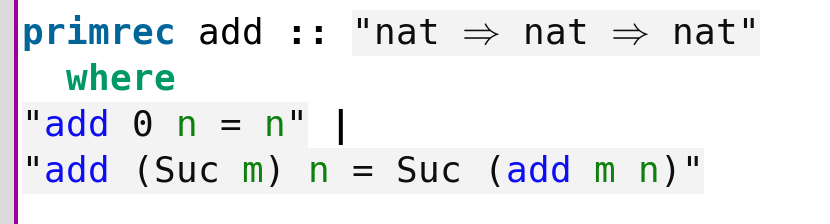
\includegraphics[scale=0.4]{images/primrec_ok.png}
  \end{frame}
  \begin{frame}
    \frametitle{Function }
    \centering
    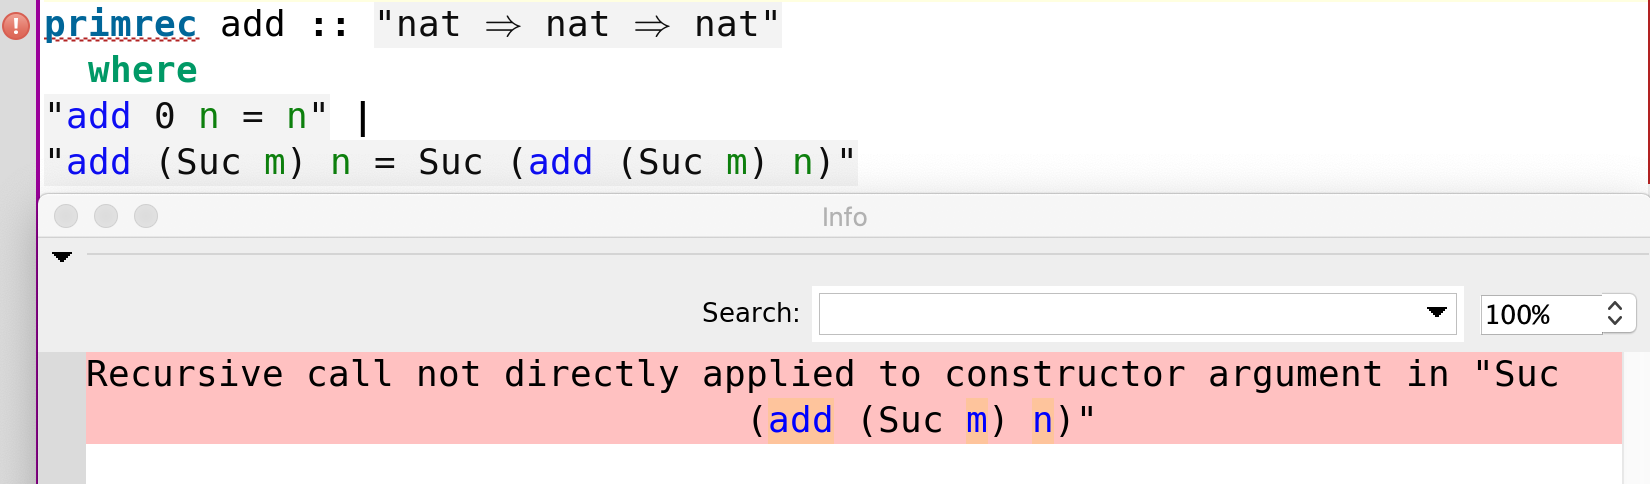
\includegraphics[scale=0.36]{images/primrec_error.png}
  \end{frame}
  \begin{frame}
    \frametitle{Function }
    \centering
    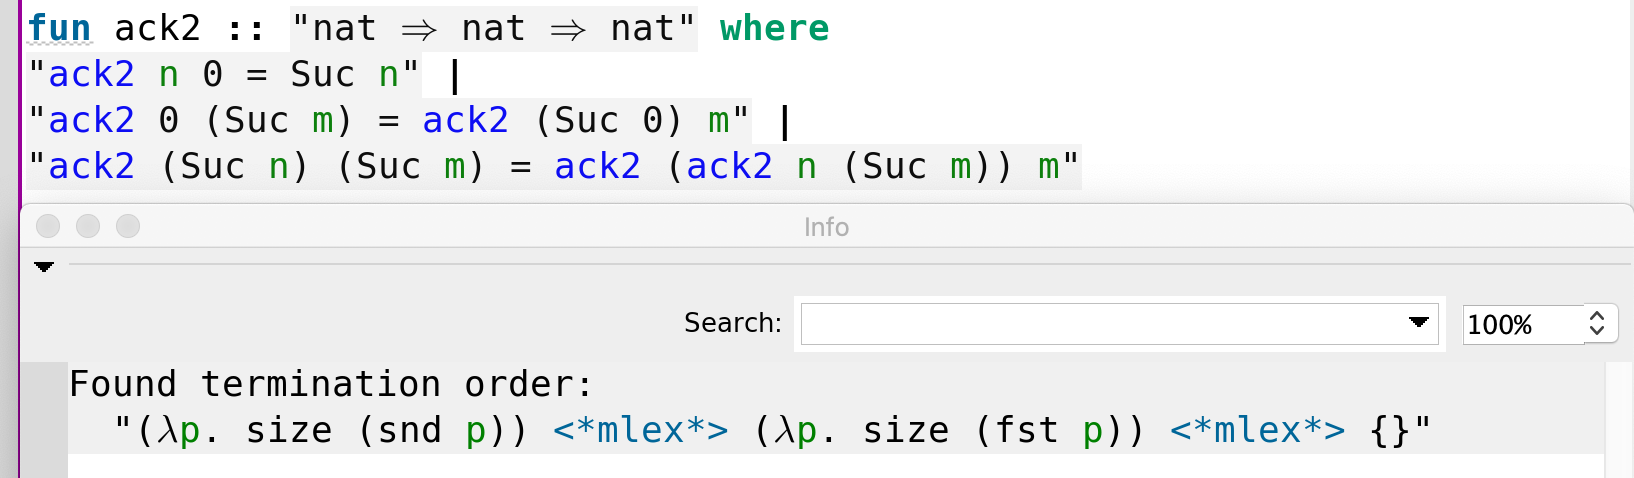
\includegraphics[scale=0.36]{images/acker_ok.png}
  \end{frame}
  \begin{frame}
    \frametitle{Function }
    \centering
    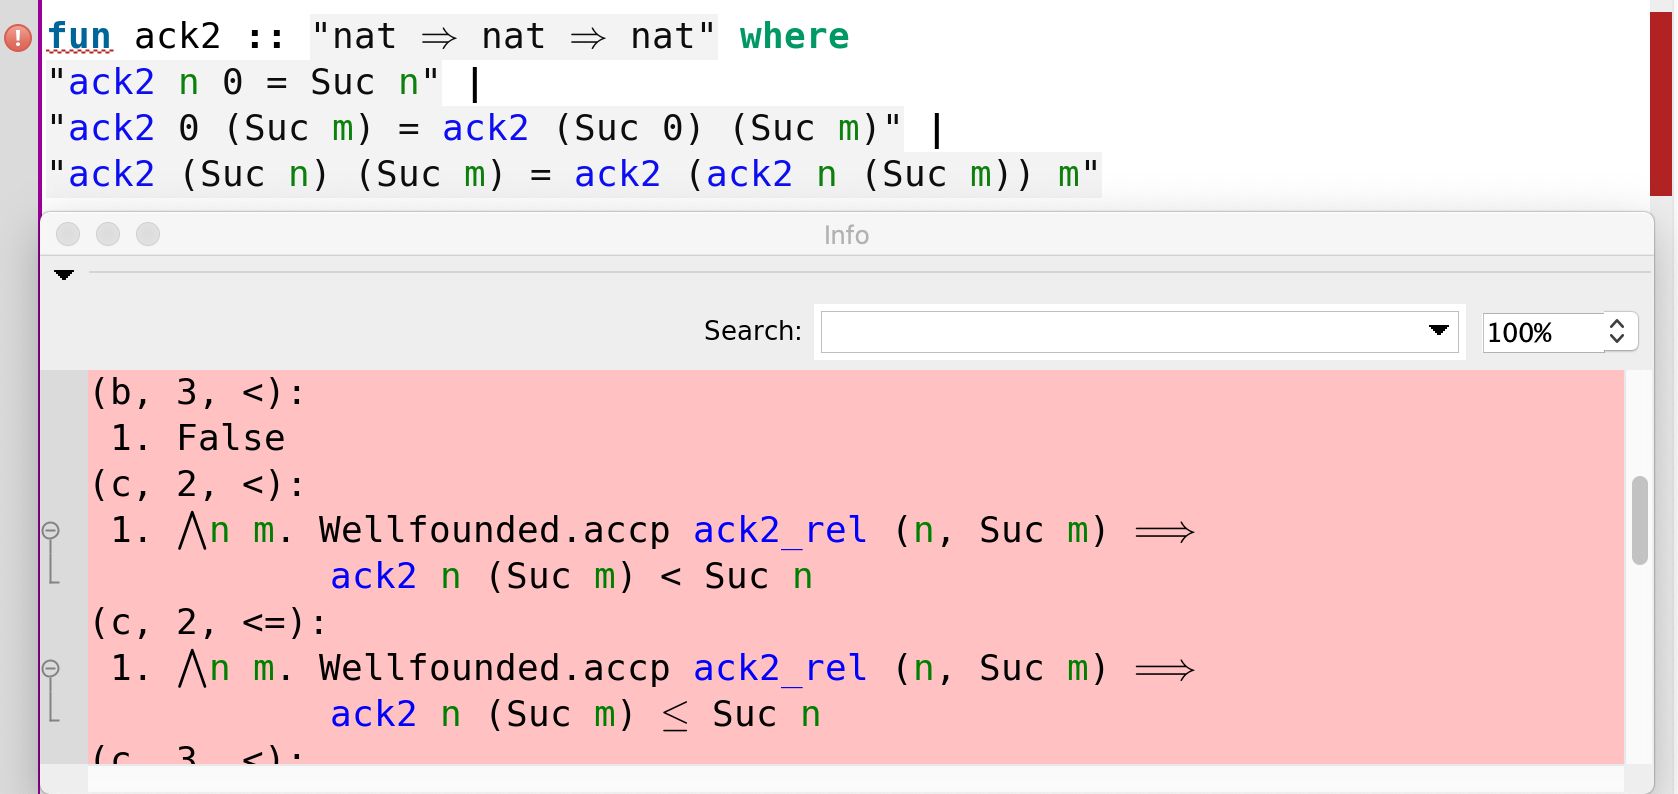
\includegraphics[scale=0.36]{images/acker_error.png}
  \end{frame}

  \begin{frame}
    \frametitle{Installation}
    Straightforward installation:
    \begin{itemize}
      \item Executable installer for Windows
      \item Bundled archive for Linux, MacOS
      \item Docker image also available\\~\

    \end{itemize}

    Installation includes an IDE tailor-made for Isabelle
    \begin{itemize}
      \item Isabelle/jEdit
    \end{itemize}
  \end{frame}

  \begin{frame}
    \frametitle{Learning Isabelle/HOL}
    \begin{itemize}
      \item Many thorough tutorials available on the Isabelle website
      (https://isabelle.in.tum.de/documentation.html)
      \item Isabelle/HOL is a functional programming language, similar to Haskell
      \item Easy to learn Isabelle/HOL if you have familiarity with functional
      programming and logic
    \end{itemize}
  \end{frame}

  \begin{frame}
    \frametitle{Live demonstration}
    We will use Isabelle/HOL to solve Assignment 2, Question 14:\\~\

    Let $\textrm{mirror} : \textrm{BinTree} \rightarrow
    \textrm{BinTree}$
    be the function that maps a binary tree to its ``mirror image''.

    \begin{enumerate}
      \item Define $\textrm{mirror}$ by pattern matching.

      \item Prove \[\forall\, t : \textrm{BinTree} \mathrel.
      \textrm{mirror}\,(\textrm{mirror}\,t) = t\] by structural
      induction.\\~\

    \end{enumerate}
  \end{frame}

\end{document}